The project was divided into two parts: \textbf{developing an automatic system} to get the TEG measurements and \textbf{fitting the data} to find the TEG parameters.
To have a complete characterization, two types of data are needed: the open-circuit voltage that is measured at the ends of the TEG when a temperature difference is applied and the current that flows through a load resistor.

The tools needed for the acquisition are the following:
\begin{itemize}
  \item The \textbf{STM32 NUCLEO-F401RE board}.
  \item The \textbf{heating and cooling control circuit board}. We used a prototype board on a matrix board.
  \item \textbf{One TEG module} with fan and heatsink on one side and the heating resistor on the other one.
  \item \textbf{Two thermocouples} (installed on the hot and cold sides). We used the \href{https://www.analog.com/media/en/technical-documentation/data-sheets/MAX6675.pdf}{MAX6675 module}.
  \item \textbf{One bench power supply} (at least rated at \(40 W\)).
  \item A PC with our \textbf{GUI application} to control MCU settings.
\end{itemize}

\begin{figure}[h]
  \centering
  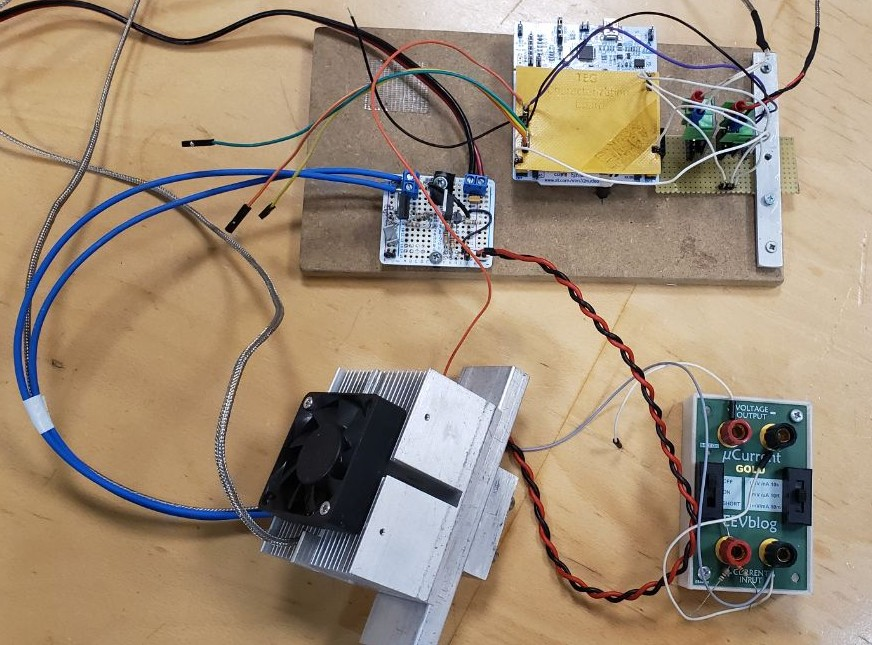
\includegraphics[width=0.45\textwidth]{assets/all_project_photo2.jpg}
  \caption{A photo of the used materials}
\end{figure}

The data acquisition procedure is organized as follows.
\begin{enumerate}
  \item Power the heating and cooling circuit, connect the STM32 NUCLEO board to the PC and open the control GUI.
  \item Set the two target temperatures from the PC and start.
  \item Save the acquired data (voltages, currents and temperatures) in CSV format on the PC.
\end{enumerate}

The STM32 uses the UART in DMA mode to communicate with the PC, the SPI to read data from the thermocouples (\href{https://www.analog.com/media/en/technical-documentation/data-sheets/MAX6675.pdf}{MAX6675 module}), the ADC to read the voltage from the TEGC, and the PWMs to control the fan and temperature of the heating resistor.

\subsection{Measurements}
TEG characterization requires us to estimate the Seebeck coefficient and the internal resistance. The method we used allowed us to estimate the two parameters with two different type of measurements.
The first one is the open-circuit voltage measurement, which allows us to estimate the Seebeck coefficient. The second one is the current measurement, which is needed to define the internal resistance. In this second test we depend on the already estimated Seebeck coefficient.

\subsection{Voltage open circuit measurement (VOC)}
\label{sec:voc-measurement}

\begin{figure}[h]
  \centering
  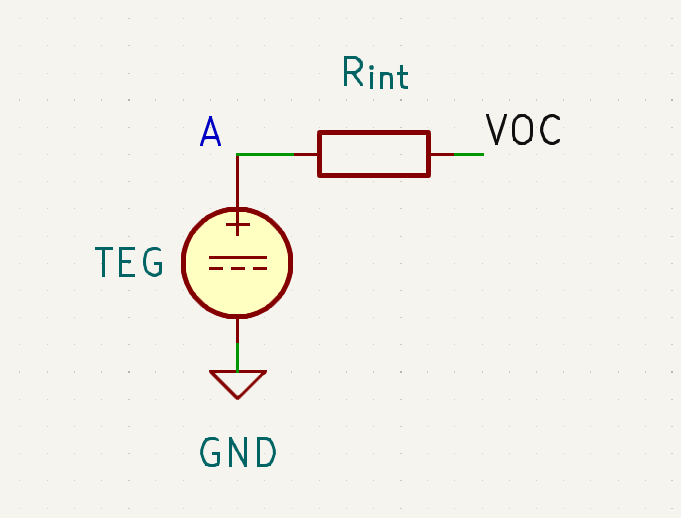
\includegraphics[width=0.45\textwidth]{assets/VOC_circuit.png}
  \caption{TEG model in open circuit configuration}
  \label{fig:oc_model}
\end{figure}
\begin{figure}[h]
  \centering
  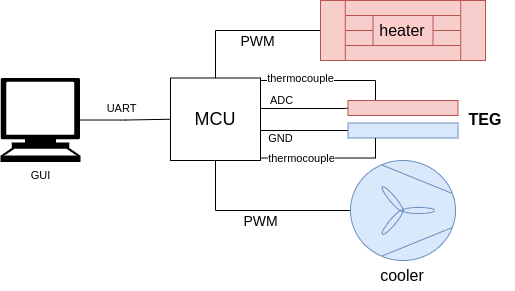
\includegraphics[width=0.45\textwidth]{assets/VOC_schema.png}
  \caption{Open circuit voltage measurement diagram}
\end{figure}

The open-circuit voltage (VOC) is the voltage measured at the ends of the TEG with no load connected, in our case, we can measure a voltage only when there is a temperature difference between the TEG surfaces.
With this test we want to measure the voltage generation of the TEG alone, and neglect the effect of the internal resistance. The only way to measure point A in figure \ref{fig:oc_model}, is to have zero current passing through $R_{int}$. To make a measurement without absorbing current, we can exploit the fact that the ADC is constructed to have high impedance, and so will limit the current to $ 5 nA $. With this in mind we can neglect this currents and assume that the measurement is done directly in point A.\\
TEG voltage is generated by the Seebeck effect, and it is proportional to the temperature difference between the hot and cold sides of the TEG, so with this test we can directly estimate the coefficient without considering other factors.
\\
The VOC is given by the following equation:

\begin{equation}
  V_{OC} = S \cdot \Delta T
  \label{eq:voc}
\end{equation}

where $ S $ is the Seebeck coefficient of the TEG and $ \Delta T $ is the temperature difference between the hot and cold sides.
The Seebeck coefficient is a material property that characterizes the voltage generated by a temperature difference, it will be used to calculate the power outut of the TEG.

\subsection{Current measurement}

\begin{figure}[h]
  \centering
  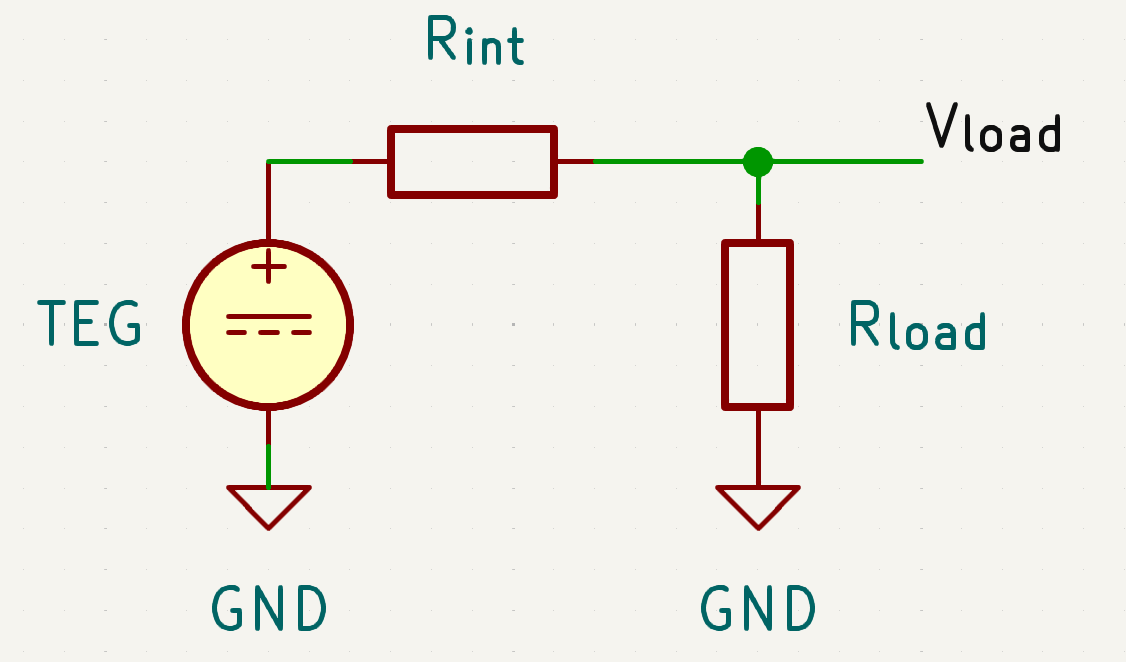
\includegraphics[width=0.45\textwidth]{assets/load_circuit.png}
  \caption{TEG model with a resistive load}
\end{figure}

The current generated by the TEG can be measured by attaching a known load resistor to the TEG and is described by the following equation:

\begin{equation}
  I = \frac{V_{OC}}{R_{int} + R_{load}}
\end{equation}

where $I$ is the current generated by the TEG, $ V_{OC} $ is the open-circuit voltage of the TEG, $ R_{int} $ is the internal resistance of the TEG, and $ R_{load} $ is the load resistor attached to the TEG.
\\
In the equation the only unknown is $R_{int}$ in fact the load resistance is chosen, $ I $ is the measured quantity and $ V_{OC} $ is instead calculated by equation \ref{eq:voc}.\\
The difficult part is to do the current measurement from the microcontroller, in fact it has no direct interface to measure it, so one way is to measure the voltage drop on a known resistance, and use $ I =  \frac{\Delta V}{R} $ to calculate the current. A shunt is a device that does this exact thing. The microcontroller's ADC has a resolution of 12 bits and the voltages are between 0 and 3.3, so, as shown here \ref{eq:adc_calculation}, the resolution is of $ 0.8 mV $.

\begin{equation}
  Resolution = \frac{3.3 V}{2^{12}} = \frac{3.3 V}{4096} = \approx 0.0008 V
  \label{eq:adc_calculation}
\end{equation}

To effectively measure we used an external module, the \href{https://www.eevblog.com/projects/ucurrent/}{\textbf{microCurrent}}, to amplify the signal then read by the MCU's ADC. This module has a tunable amplification circuit that allows to change the expected scale and resolution to fit the expected currents range.

\begin{figure}[h]
  \centering
  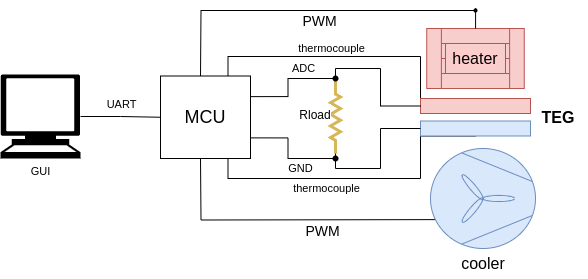
\includegraphics[width=0.45\textwidth]{assets/load_schema.png}
  \caption{Current measurement diagram with a resistive load}
\end{figure}


\subsection{Hot side temperature control}

\begin{figure}
  \centering
  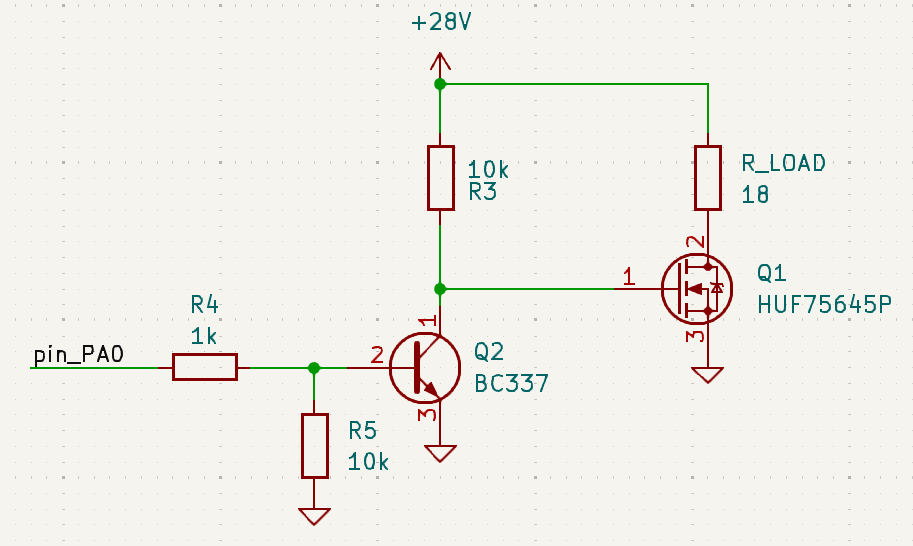
\includegraphics[width=0.45\textwidth]{assets/heat_control.png}
  \caption{Current control circuit}
  \label{fig:heat_control}
\end{figure}

For every measurement we need a temperature difference between the two sides of the TEG, so we
need to control the temperature of the hot side.
We used a \textbf{wire wound resistor with a current control}. The circuit (in Figure \ref{fig:heat_control}) involves a \href{https://www.onsemi.com/pdf/datasheet/huf75645s3s-d.pdf}{MOSFET} driven by a \href{https://diotec.com/request/datasheet/bc337.pdf}{NPN transistor}. As a load resistor we used a wire wound resistor of 18 effective ohms (measured with the multimeter). Both SPICE simulation and actual measurements confirm a maximum current of $ 1.4 A $ on the load resistor, with a maximum power around $ 35 W $ as shown here \ref{eq:power_supply_rating}. \\

\begin{equation}
  (1.4A)^2 * 18\Omega = 35W
  \label{eq:power_supply_rating}
\end{equation}

The circuit has reverse logic, so when the MCU pin is grounded the mosfet is activated and 1.4 A of current flows through, but when it is at 3.3V it stops. R3 and R5 are chosen according to this configuration, R4 is only a protection resistor for the MCU pin.


\subsection{Cold side temperature control}

To maintain a constant temperature, a \textbf{heatsink} was positioned on the cold side of the TEG. Subsequently, a fan was incorporated into the system to facilitate cooling of the aluminum, which proved particularly advantageous during steady-state acquisitions. This approach enabled the temperature of the hot side to be maintained at a stable level through the PID on the heater, the temperature of the cold side to be kept stable by the fan, and the delta to remain constant. A 12V fan with a PWM control was utilized. The power supply was the same as that used for the heater, and a \href{https://www.ti.com/lit/ds/symlink/lm317l.pdf}{voltage regulator} with the appropriate resistors was employed to provide a 12V power supply. The PID was tuned to control the fan, but we found out that it was preferable to run the fan constantly in steady-state measurements or to turn it off in measurements with equal delta temperatures but different average temperatures. 

\begin{figure}[h]
  \centering
  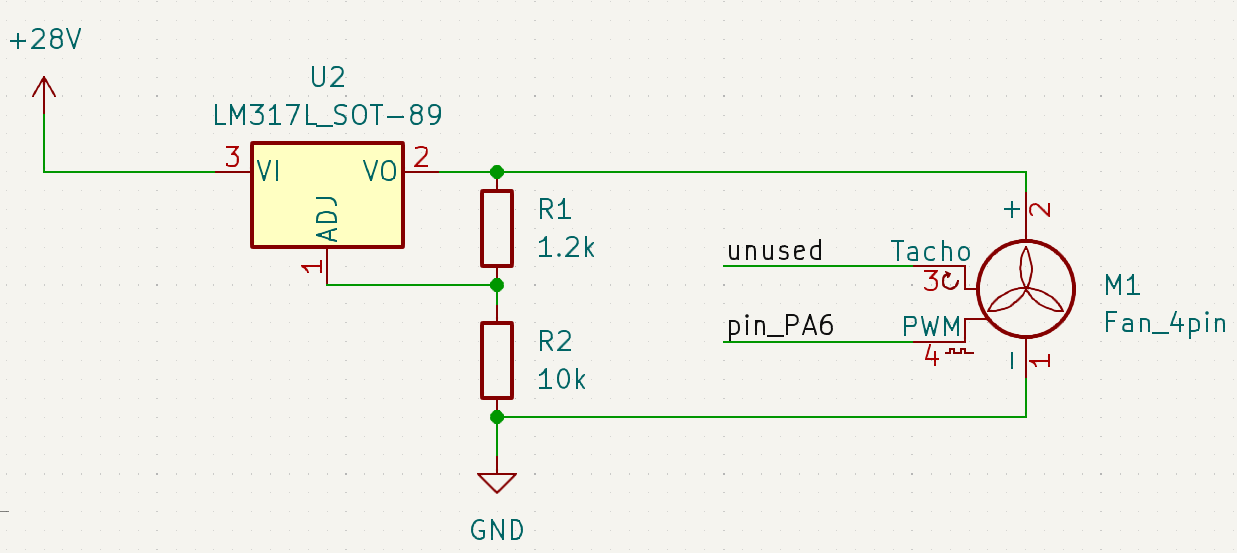
\includegraphics[scale=0.25]{assets/cooling_control.png}
  \caption{Cooling control circuit}
\end{figure}

\subsection{Acquisition process}

The MCU accepts via UART the following commands:
\begin{itemize}
  \item \textbf{setpoint hot\_side}: set the hot side temperature in Celsius degrees
  \item \textbf{duty duty\_cycle}: set the duty cycle of the PWM controlling the fan, from 0 to 1
  \item \textbf{pid kp ki kd}: set the PID parameters
\end{itemize}

The GUI application was developed in C++ using the \href{https://github.com/ocornut/imgui}{\textbf{Dear ImGui}} library and it allows to control the MCU parameters, plot the acquired data and save it in CSV format.

\begin{figure}[h]
  \centering
  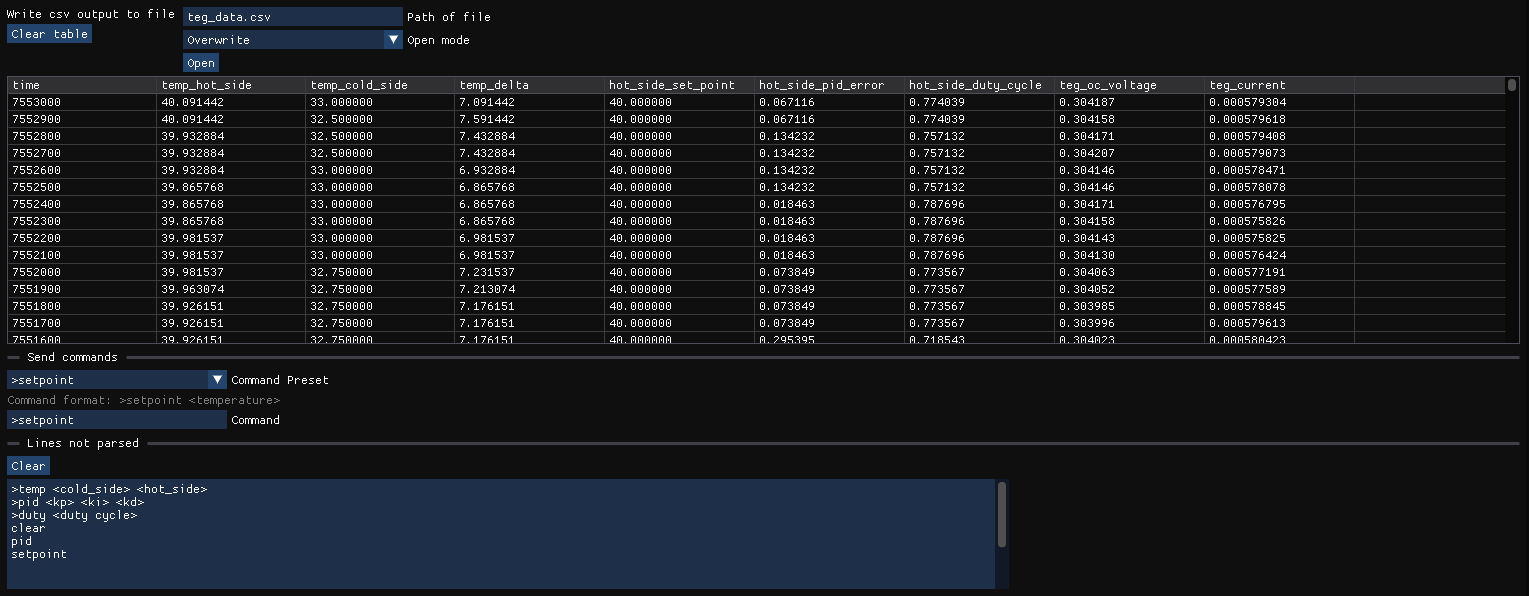
\includegraphics[width=0.5\textwidth]{assets/app_csv_commands.png}
  \caption{Sending the settings to the MCU}
\end{figure}

We carried out the acquisitions in the same environment, thus maintaining the same conditions for all acquisitions. We justify the time used for the development of the application as it was very useful both for acquiring accurate data and for quickly noticing any errors or dirty data so that we could stop and correct, saving time later.

\begin{figure}[h]
  \centering
  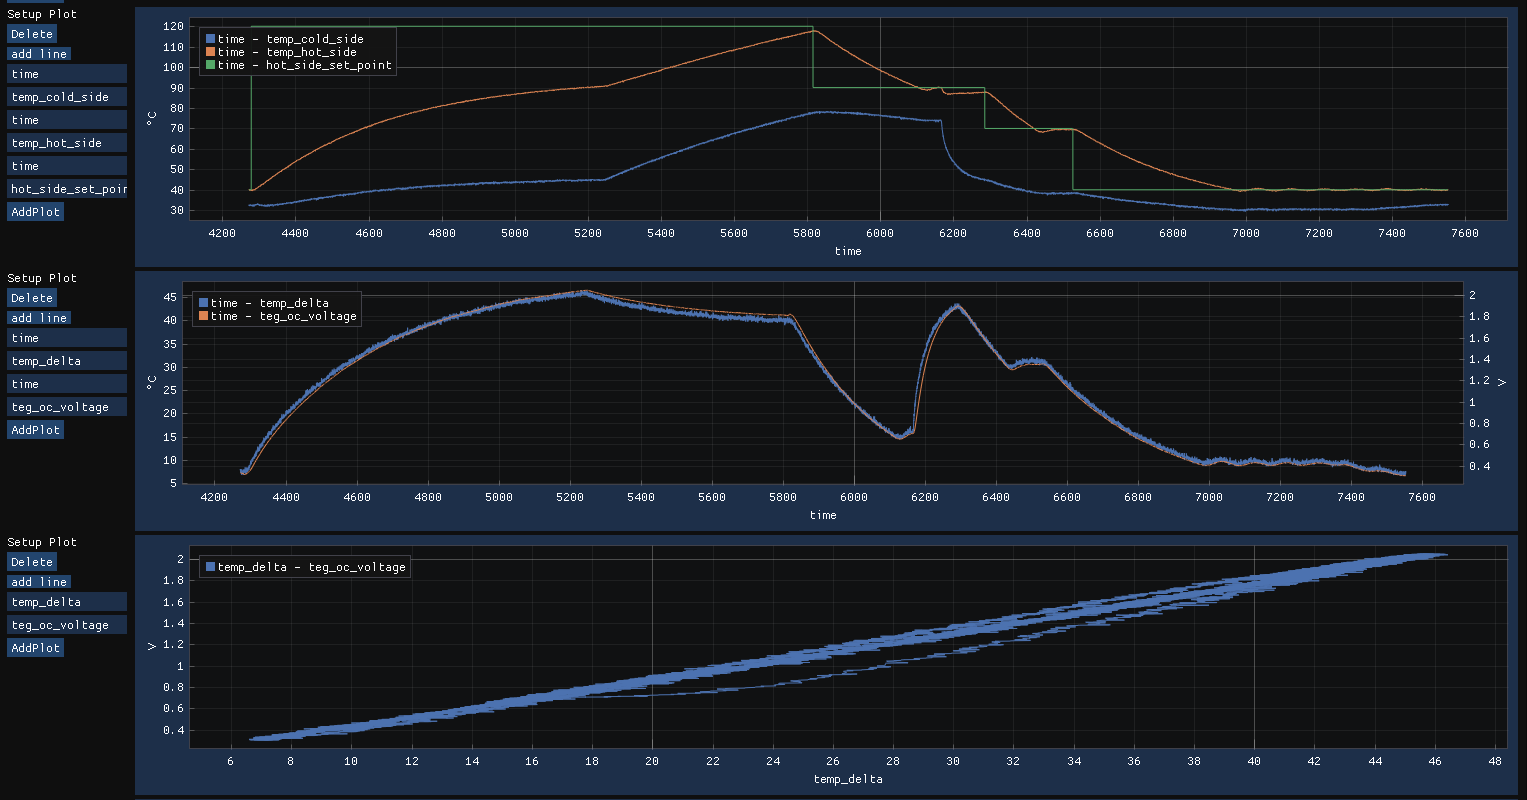
\includegraphics[width=0.5\textwidth]{assets/app_plots.png}
  \caption{Real time plots from the GUI application}
\end{figure}


